\chapter{INTRODUÇÃO}

Texto (SOBRENOME, ano).

\section{Seção}

Texto, conforme a Figura~\ref{fig:example_1}.

\begin{figure}[H]
    \centering
    \caption{Título da figura.}
    \label{fig:example_1}
    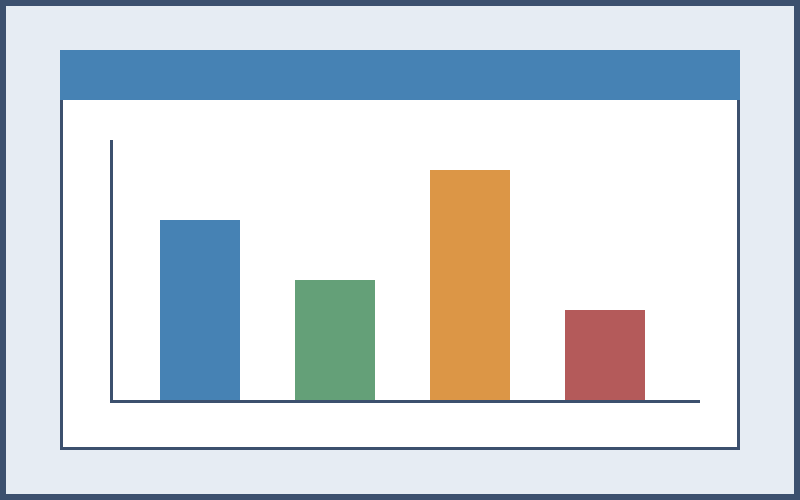
\includegraphics[width=0.9\textwidth]{images/example.png}
    \authorssource
\end{figure}

\subsection{Subseção}

Texto:

\begin{itemize}
    \item Item;
    \item Item.
\end{itemize}

\section{Seção}

Texto, conforme a Tabela~\ref{tab:example} e o Quadro~\ref{frame:example_1}.

\begin{center}
\captionof{tabela}{Título da tabela}
\label{tab:example}
\begin{tabular}{lrr}
\toprule
\textbf{Coluna 1} & \textbf{Coluna 2} & \textbf{Coluna 3} \\
\midrule
Linha 1 & 0 & 0,0\% \\
Linha 2 & 0 & 0,0\% \\
\bottomrule
\end{tabular}
\authorssource
\end{center}

\begin{table}[H]
\centering
\caption{Título do quadro}
\label{frame:example_1}
\begin{tabular}{|c|p{10cm}|}
\hline
\textbf{Coluna 1} & \textbf{Coluna 2} \\ \hline
1 & Texto \\ \hline
2 & Texto \\ \hline
\end{tabular}

\authorssource
\end{table}
